Initially, we set the Reorder Buffer (ROB) size to 24. However, this led to a noticeable performance issue: around 12\% of instructions encountered structural hazards during dispatch due to ROB entries being unavailable. As a result, pipeline stalls and the overall CPI is high.

To address this bottleneck, we experimented with resizing the ROB. Our results in Fig. \ref{fig:rob_stall} show that increasing the ROB size significantly reduced structural hazards—by approximately 50\%—which in turn lowered the CPI by 0.8\%, as shown in Fig. \ref{fig:rob_cpi}.
\begin{figure}[htbp]
  \centering
  \begin{minipage}[t]{0.24\textwidth}
    \centering
    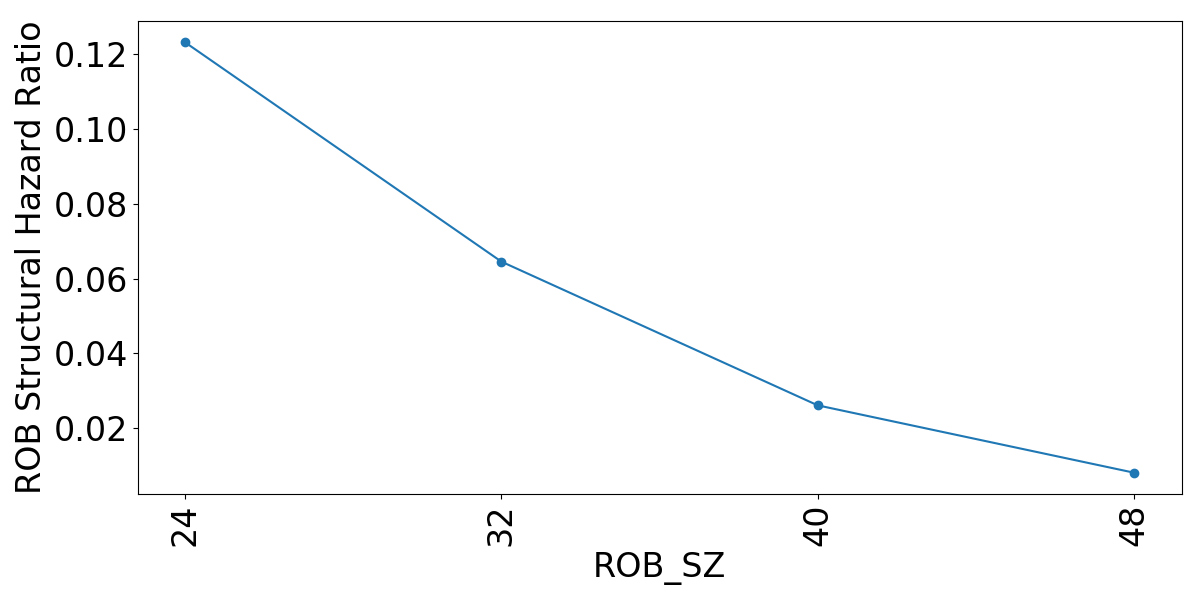
\includegraphics[width=\textwidth]{figures/Analysis/N-way/ROB_Stru.png}
    \caption{ROB Size vs. ROB Full Rate}
    \label{fig:rob_stall}
  \end{minipage}
  \hfill
  \begin{minipage}[t]{0.24\textwidth}
    \centering
    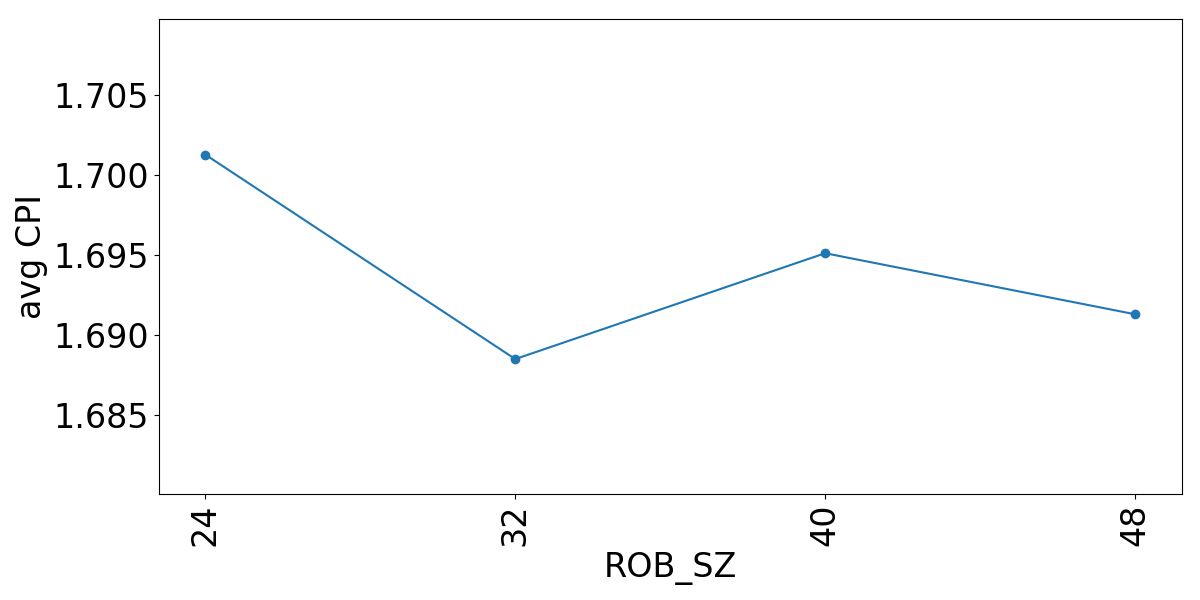
\includegraphics[width=\textwidth]{figures/Analysis/N-way/cpi_ROB.png}
    \caption{ROB Size vs. CPI}
    \label{fig:rob_cpi}
  \end{minipage}
\end{figure}
However, we also observed that beyond a certain point, further increasing the ROB size led to higher CPI. We hypothesize that this is because when too many instructions are waiting to be issued, backend resources become saturated. This causes newer instructions to occupy resources needed by older instructions, preventing them from completing and introducing stalls in a different part of the pipeline. Therefore, we finalized our ROB size to 32, and our ROB full rate is about 6\%.